\subsection{Autonomous Paper-Production Case Study}
\label{sec:paper-case-study}

The benchmark suite evaluates task endpoints, while the mathematical trace follows
one research objective in depth. A complementary question is whether the same
runtime can carry multiple research programs through the complete paper-production
lifecycle. We therefore reconstruct six projects spanning evaluation reliability,
vision--language matching, test-time adaptation, GUI agents, multimodal
hallucination, and model quantization. The initial objectives and compute
environments were provided externally; the retained Argus records identify the
Manager, Planner, Engineer, and Reviewer as the actors responsible for Stage
transitions, experiments, manuscript construction, review, and submission checks.

Figure~\ref{fig:paper-case-study} summarizes the portfolio. All
\PaperCaseCompleted{} of \PaperCasePapers{} canonical pipelines reach the final
submission Stage. In aggregate, they span \PaperCaseCampaignHours{} campaign-hours,
\PaperCaseMissions{} bounded missions, \PaperCaseRounds{} Engineer rounds,
\PaperCaseContinues{} Reviewer revision verdicts, \PaperCaseSessionRolls{} session
rolls, and \PaperCaseRollbacks{} Manager rollbacks. Campaign-hours are summed across
projects and are not calendar time because several projects overlap.

\begin{figure}[H]
  \centering
  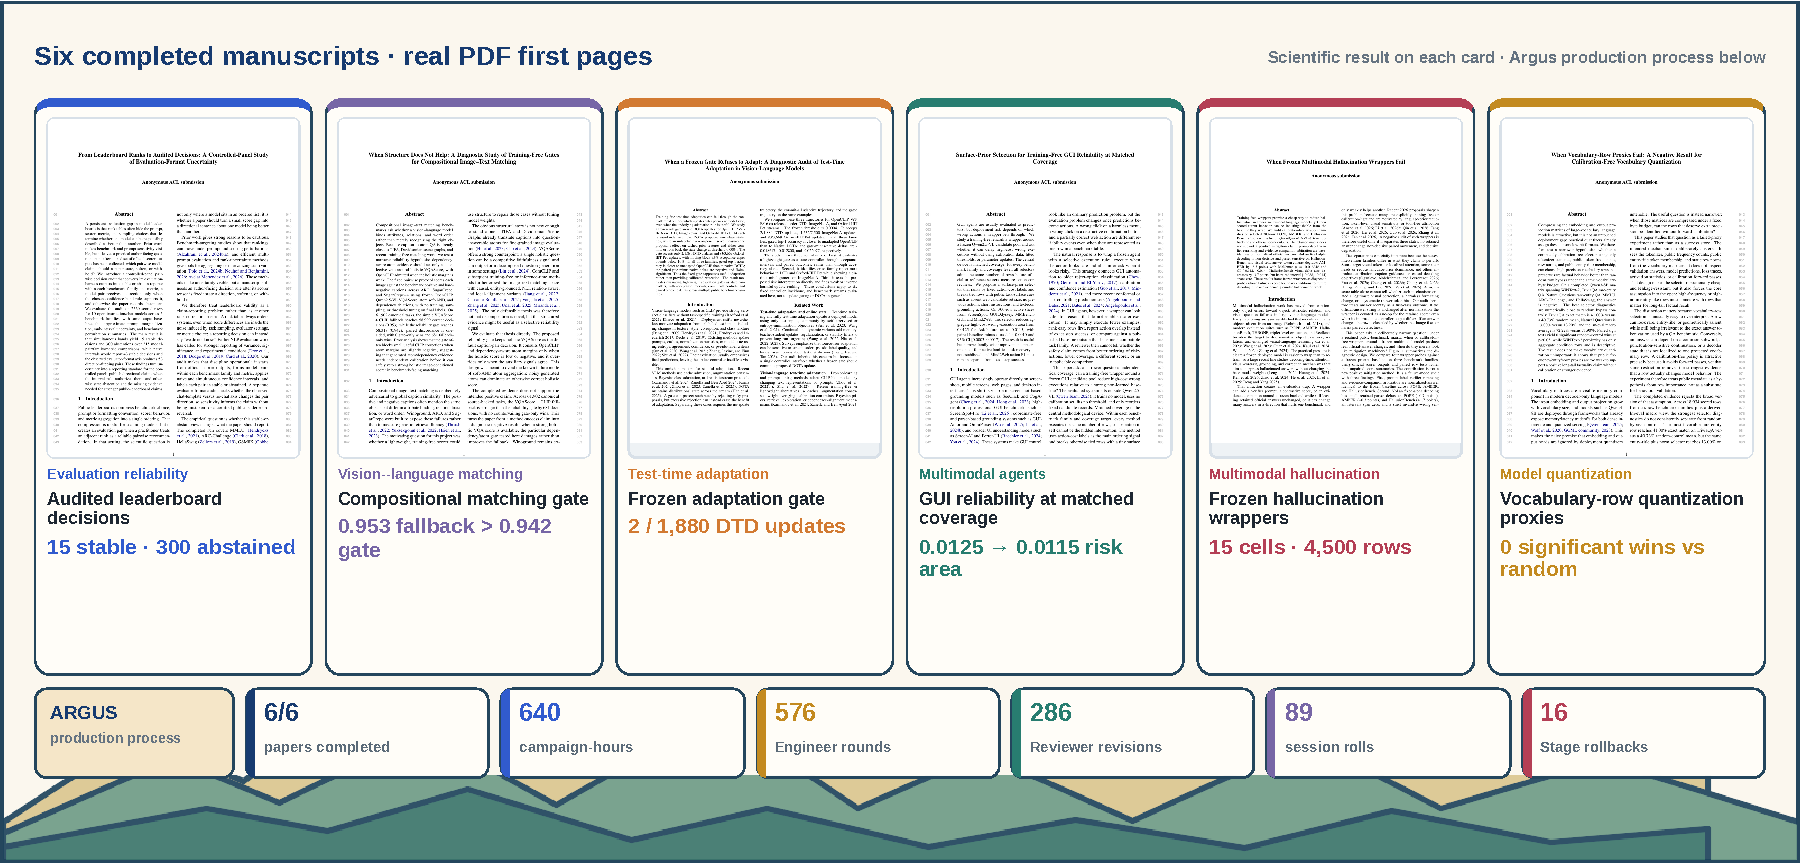
\includegraphics[width=\linewidth]{figures/paper_case_study.pdf}
  \caption{One recurrent runtime, six scientific outputs. Panel (a)
  schematizes the four role authorities around persistent research state. Panel
  (b) reports the research topic and principal measured finding from each
  final manuscript. The bottom strip aggregates structured runtime events across
  the six campaigns. The mechanism panel is schematic; the paper findings and
  process counts are measured. AAAI and ACL labels denote formatting rather than
  venue acceptance.}
  \label{fig:paper-case-study}
\end{figure}

The trajectories are inconsistent with a one-pass account of autonomous paper
writing. Each manuscript states a scoped research question and a task-native
outcome rather than merely presenting a generated document. The portfolio includes
uncertainty-aware leaderboard reporting, a failed compositional gate, an
over-restrictive adaptation controller, a narrow GUI reliability gain, a
failure-mode audit of multimodal wrappers, and a negative result for static
quantization proxies. Several projects therefore become diagnostic or negative
results after their original positive hypothesis fails. Reviewer-gated state makes
that scientific pivot explicit instead of silently replacing the failed branch.

Figure~\ref{fig:paper-case-trajectory} resolves the multimodal-hallucination
campaign in greater detail. During a dense 12-hour search window, seven rollback
decisions reject baseline coverage or proposed mechanisms that are unreproduced,
base-identical, or missing their preregistered signal. Planner then changes the
claim from a positive mitigation method to a diagnostic negative-results audit.
Engineer completes a five-method by three-benchmark matrix with 4,500
official-scored rows; Reviewer binds the resulting no-op and degradation claims to
those outputs. Two later submission checks return the project to benchmark to
repair scorer provenance and GPU telemetry before the final 10-page AAAI-formatted
package completes the pipeline.

\begin{figure}[H]
  \centering
  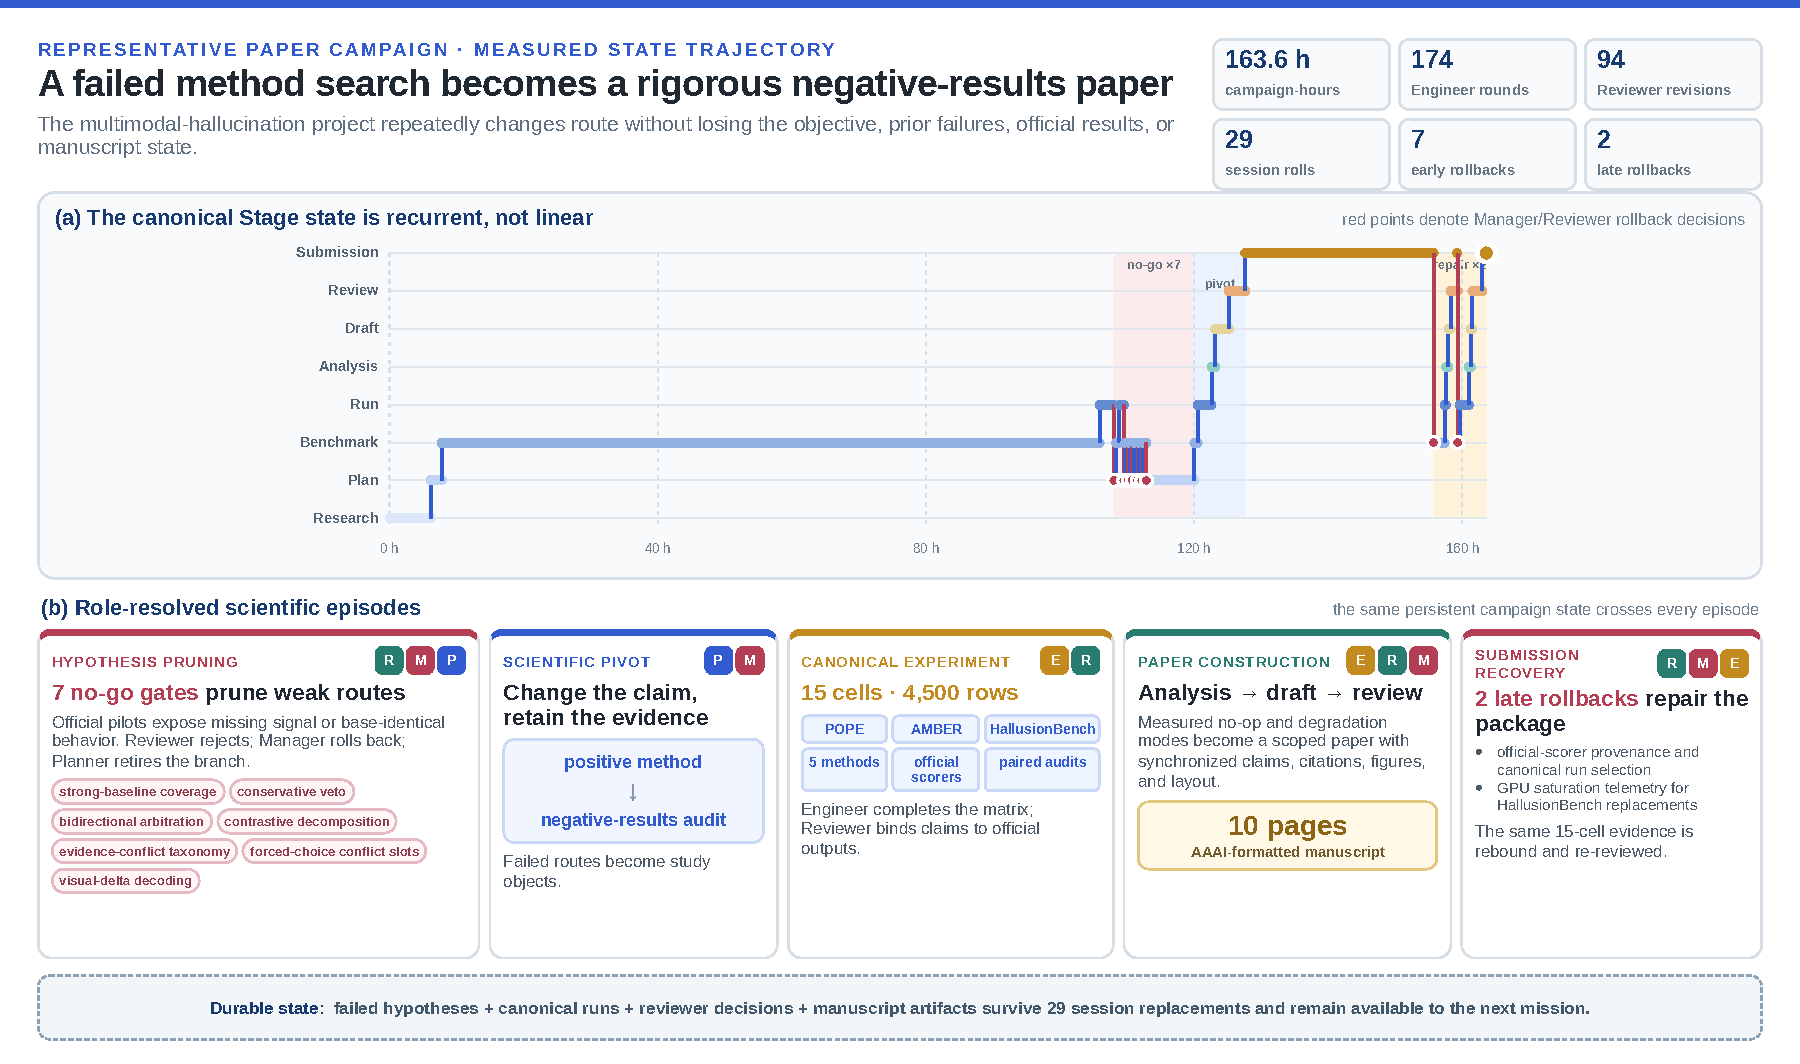
\includegraphics[width=\linewidth]{figures/paper_case_trajectory.pdf}
  \caption{Representative 163.6-hour paper-production trajectory. The upper panel
  plots the actual Manager-controlled Stage state against elapsed campaign-hours;
  red points mark rollback decisions. Seven early no-go rollbacks prune weak method
  routes before a negative-results scope pivot, and two submission-to-benchmark
  rollbacks repair the final evidence package. The lower panel identifies the role
  actions and retained artifacts at each scientific episode. The canonical
  experiment contains 15 method--benchmark cells and 4,500 official-scored rows;
  29 session rolls do not reset the campaign state.}
  \label{fig:paper-case-trajectory}
\end{figure}

The process layer is similarly nontrivial. Even the shortest case requires 28
Engineer rounds, 19 Reviewer revisions, and 13 session rolls over 20.8 hours. The
two AAAI-formatted cases finish as 10-page anonymous submissions, while the four
ACL-formatted cases contain 10--13 pages. Across all six projects, the retained
academic, layout, and infrastructure histories contain
\PaperCaseReviewSnapshots{} automated review snapshots. These are process records
rather than external assessments of paper quality.

The case study also exposes a consistency failure. The compositional-matching
pipeline reaches a complete submission Stage and produces its final PDF, while the
last stored assurance object remains \code{BLOCKED} on a Manager-stage authority
check. This discrepancy does not change the paper artifact, but it shows that
derived certification state can lag the canonical pipeline state. Public release
automation should reconcile those two views before presenting assurance as a final
verdict.
